\documentclass[border=8pt]{standalone}
\usepackage{tikz}
\usepackage{amsmath,amssymb}
\usetikzlibrary{arrows.meta,positioning,shapes.geometric,fit,calc,decorations.pathreplacing,backgrounds}

\definecolor{cprimary}{HTML}{2D5F8A}
\definecolor{cprimarylight}{HTML}{5B8DB8}
\definecolor{csecondary}{HTML}{C25B28}
\definecolor{csecondarylight}{HTML}{E8925F}
\definecolor{caccent}{HTML}{3A8C6E}
\definecolor{caccentlight}{HTML}{6BB89A}
\definecolor{cwarning}{HTML}{D4A843}
\definecolor{cneutraldark}{HTML}{333333}
\definecolor{cneutralmid}{HTML}{888888}
\definecolor{cneutrallight}{HTML}{CCCCCC}
\definecolor{bgencoder}{HTML}{E8F0F8}
\definecolor{bgpredictor}{HTML}{FFF3E8}
\definecolor{bgtarget}{HTML}{E8F8F0}
\definecolor{bgloss}{HTML}{FFF8E8}
\definecolor{bgpast}{HTML}{DDEAF6}
\definecolor{bgfuture}{HTML}{DEF0E8}
\definecolor{carrow}{HTML}{555555}

\begin{document}
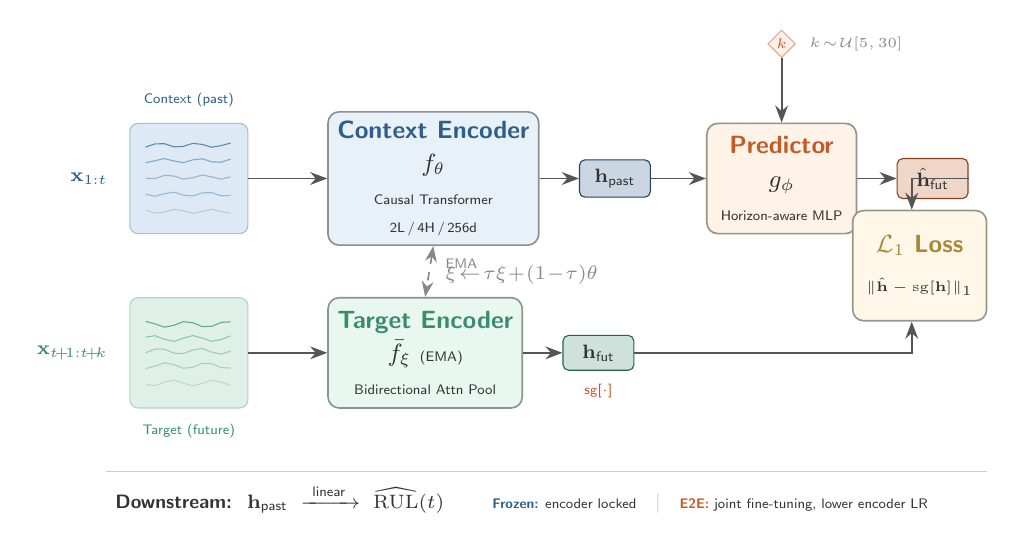
\begin{tikzpicture}[
    >=Stealth,
    font=\sffamily\small,
    block/.style={
        rounded corners=4pt,
        draw=#1!60!black,
        line width=0.6pt,
        fill=#1,
        minimum height=1.4cm,
        minimum width=2.0cm,
        align=center,
        text=cneutraldark
    },
    vec/.style={
        rounded corners=2pt,
        draw=#1!70!black,
        fill=#1!25,
        minimum height=0.36cm,
        minimum width=0.9cm,
        align=center,
        font=\sffamily\scriptsize,
        text=cneutraldark
    },
    dataarrow/.style={->,line width=0.7pt,carrow},
    brace/.style={decorate,decoration={brace,amplitude=4pt,raise=2pt}},
]

% ============================================================
% COLUMN 1: Input time series (left)
% ============================================================

% Past
\node[
    rounded corners=3pt, draw=cprimary!40, fill=bgpast,
    minimum height=1.4cm, minimum width=1.5cm,
] (past) at (0,0) {};

\foreach \yoff/\col in {0.4/cprimary,0.2/cprimarylight,0.0/cprimary!60,
                        -0.2/cprimarylight!80,-0.4/cprimary!40} {
    \draw[thin,\col,opacity=0.7] ([xshift=-0.55cm,yshift=\yoff cm]past.center)
        \foreach \x in {0,0.12,...,1.0} { -- ++(0.12,{0.04*sin(\x*800+\yoff*200)}) };
}

% Future (below past)
\node[
    rounded corners=3pt, draw=caccent!40, fill=bgfuture,
    minimum height=1.4cm, minimum width=1.5cm,
    below=0.8cm of past,
] (future) {};

\foreach \yoff/\col in {0.4/caccent,0.2/caccentlight,0.0/caccent!60,
                        -0.2/caccentlight!80,-0.4/caccent!40} {
    \draw[thin,\col,opacity=0.7] ([xshift=-0.55cm,yshift=\yoff cm]future.center)
        \foreach \x in {0,0.12,...,1.0} { -- ++(0.12,{0.05*sin(\x*700+\yoff*300+100)}) };
}

% Labels
\node[font=\sffamily\scriptsize,cprimary,left=0.15cm of past] {$\mathbf{x}_{1:t}$};
\node[font=\sffamily\tiny,cprimary,above=0.08cm of past] {Context (past)};
\node[font=\sffamily\scriptsize,caccent,left=0.15cm of future] {$\mathbf{x}_{t\!+\!1:t\!+\!k}$};
\node[font=\sffamily\tiny,caccent,below=0.08cm of future] {Target (future)};

% ============================================================
% COLUMN 2: Encoders (two parallel branches)
% ============================================================

% Context Encoder (top branch)
\node[block=bgencoder,minimum width=2.2cm,right=1.0cm of past] (encoder) {
    \textbf{\textcolor{cprimary}{Context Encoder}}\\[1pt]
    $f_\theta$\\[1pt]
    {\tiny Causal Transformer}\\[-1pt]
    {\tiny 2L\,/\,4H\,/\,256d}
};
\draw[dataarrow] (past.east) -- (encoder.west);

% Target Encoder (bottom branch)
\node[block=bgtarget,minimum width=2.2cm,right=1.0cm of future] (target) {
    \textbf{\textcolor{caccent}{Target Encoder}}\\[1pt]
    $\bar{f}_\xi$ {\tiny (EMA)}\\[1pt]
    {\tiny Bidirectional Attn Pool}
};
\draw[dataarrow] (future.east) -- (target.west);

% EMA connection between encoders (short vertical dashed arrow)
\draw[<->,line width=0.6pt,cneutralmid,dashed]
    (encoder.south) -- (target.north)
    node[midway,right=0.08cm,font=\sffamily\tiny,cneutralmid,align=left]
    {EMA\\[-2pt]{\scriptsize$\xi \!\leftarrow\! \tau\xi\!+\!(1\!-\!\tau)\theta$}};

% ============================================================
% COLUMN 3: Representations
% ============================================================

% h_past
\node[vec=cprimary,right=0.5cm of encoder.east] (hpast) {$\mathbf{h}_\text{past}$};
\draw[dataarrow] (encoder.east) -- (hpast.west);

% h_future (with stop-gradient)
\node[vec=caccent,right=0.5cm of target.east] (hfut) {$\mathbf{h}_\text{fut}$};
\draw[dataarrow] (target.east) -- (hfut.west);
\node[font=\sffamily\tiny,csecondary,below=0.04cm of hfut] {\textsf{sg}[$\cdot$]};

% ============================================================
% COLUMN 4: Predictor (bridges top branch to comparison)
% ============================================================

\node[block=bgpredictor,right=0.7cm of hpast.east,anchor=west,minimum width=1.9cm] (predictor) {
    \textbf{\textcolor{csecondary}{Predictor}}\\[1pt]
    $g_\phi$\\[1pt]
    {\tiny Horizon-aware MLP}
};
\draw[dataarrow] (hpast.east) -- (predictor.west);

% Horizon k (small, above predictor)
\node[
    diamond, draw=csecondary!50, fill=csecondarylight!15,
    minimum size=0.35cm, inner sep=0pt,
    font=\sffamily\tiny, text=csecondary
] (horizon) at ([yshift=1.0cm]predictor.north) {$k$};
\draw[dataarrow] (horizon.south) -- (predictor.north);
\node[font=\sffamily\tiny,cneutralmid,right=0.05cm of horizon] {$k\!\sim\!\mathcal{U}[5,30]$};

% h_hat_future
\node[vec=csecondary,right=0.5cm of predictor.east] (hfuthat) {$\hat{\mathbf{h}}_\text{fut}$};
\draw[dataarrow] (predictor.east) -- (hfuthat.west);

% ============================================================
% COLUMN 5: Loss (compares predicted vs target)
% ============================================================

\node[
    block=bgloss,
    minimum width=1.7cm,
    minimum height=1.4cm,
] (loss) at ([xshift=1.5cm]$(hfuthat.east)!0.5!(hfut.east)$) {
    \textbf{\textcolor{cwarning!80!black}{$\mathcal{L}_1$ Loss}}\\[3pt]
    {\tiny $\|\hat{\mathbf{h}} - \mathrm{sg}[\mathbf{h}]\|_1$}
};

% h_hat -> loss (from above-left)
\draw[dataarrow] (hfuthat.east) -| ([xshift=-0.1cm]loss.north);

% h_fut -> loss (from below-left)
\draw[dataarrow] (hfut.east) -| ([xshift=-0.1cm]loss.south);

% ============================================================
% DOWNSTREAM ANNOTATION (below everything)
% ============================================================

\coordinate (bleft) at ([xshift=-0.3cm]past.west);
\coordinate (bright) at (loss.east);

\draw[cneutrallight,line width=0.3pt]
    ([yshift=-0.8cm]future.south -| bleft) -- ([yshift=-0.8cm]future.south -| bright);

\node[font=\sffamily\scriptsize,cneutraldark,anchor=west]
    at ([yshift=-1.15cm]future.south -| bleft) {
    \textbf{Downstream:}\;
    $\mathbf{h}_\text{past} \;\xrightarrow{\;\text{linear}\;}\; \widehat{\mathrm{RUL}}(t)$
    \qquad
    {\tiny\textcolor{cprimary}{\textbf{Frozen:}} encoder locked}
    \;\;\textcolor{cneutrallight}{$\vert$}\;\;
    {\tiny\textcolor{csecondary}{\textbf{E2E:}} joint fine-tuning, lower encoder LR}
};

\end{tikzpicture}
\end{document}
